\documentclass{article}

\usepackage{graphicx}
\usepackage{array}
\usepackage[group-separator={,}]{siunitx}
\usepackage{authblk}	% prettier multiple authors
\usepackage{tikz}

\usepackage[margin=0.75cm]{caption}
\usepackage{hyperref}

% see http://texblog.org/2008/05/07/fwd-equal-cell-width-right-and-centre-aligned-content/
\newcolumntype{x}[1]{%
>{\centering\hspace{0pt}}p{#1}}%

\title{Real-Time Social Data Sampling }
\author[]{Scott Hendrickson}
\author[]{Brian Lehman}
\author[]{Joshua Montague}
\affil[]{ \Large{Gnip, Inc.} }

\begin{document}
\maketitle

\frenchspacing

%%%%%%%%%%%%%%%%%%%%%%%%%%%%%%%%%%
\section{Introduction}
\label{intro}


% keep this code at the top of the Introduction to ensure the figure stays on page 1
%%%%%
% figure
%
\begin{figure}[!b]
\begin{center}
% http://cremeronline.com/LaTeX/minimaltikz.pdf
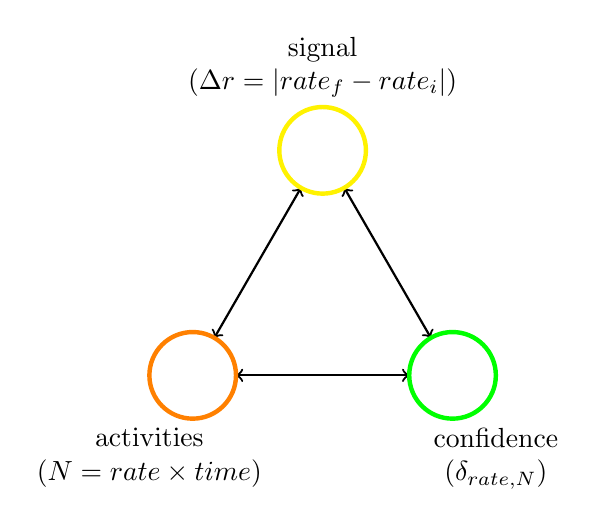
\begin{tikzpicture}[scale=1.1]]
% arrows
\draw [thick, <->] (0.25000000000000006, 0.4330127018922193) -- (1.25, 2.165063509461097) ;
\draw [thick, <->] (1.75, 2.165063509461097) -- (2.75, 0.4330127018922193) ;
\draw [thick, <->] (2.5, 0) -- (0.5, 0) ;
% circles
\draw [orange, ultra thick] (0,0) circle [radius=0.5];
\draw [yellow, ultra thick] (1.5,2.598) circle [radius=0.5];
\draw [green, ultra thick] (3,0) circle [radius=0.5];
% labels
\node[align=center, below] at (-0.5,-0.5){activities\\($N=rate \times time$)};
\node[align=center, above] at (1.5,3.098){signal\\($\Delta r=|rate_f-rate_i|$)};
\node[align=center, below] at (3.5,-0.5){confidence\\($\delta_{rate,N}$)};
\end{tikzpicture}
\end{center}
\caption{The three parameters used in classifying signal from real-time data: signal size, 
total activities, and confidence. Signal size is a change in activity rate, the total 
number of activities observed is a function of observation time, and confidence is that of a reported 
activity rate. These parameters are not simultaneously independent; we can choose or measure 
any two and then calculate the third.}
\label{fig:tradeoff}
\end{figure}
%
%
%%%%%


In the world of real-time social data, we are typically observing a series of activities during some 
period of time and are interested in identifying significant changes in the corresponding activity 
rate. Such changes may be signals of emerging events or conversations. In this work, 
we hope to assist current and potential Gnip customers in 
% thesis statement: help our customers better understand a) how to use PT b) how to set up their measurements

we would like to quantify our ability to identify these kinds of signals. Figure~\ref{fig:tradeoff} 
illustrates (schematically) the three main parameters involved in such calculations: signal size, total 
activities, and confidence. The three parameters are not simultaneously independent; we can 
choose or measure two of them -- possibly based on our particular use-case -- and they will 
determine the third. If chosen as \emph{ad hoc} parameters, respectively, the signal 
size is a difference in activity rates between two observation times, the number of total 
activities is a function of the observation time and underlying instantaneous activity rate, and the 
confidence is a measure of statistical uncertainty in the activity rate e.g. a 95$\%$ 
confidence interval.

For popular topics, social media streams contain a sufficient rate of activities e.g. blog posts or 
Tweets to create reliable, high-resolution signals in short observation times.  
However, less popular topics with infrequent activities require additional effort in order to adequately 
determine the number of activities, signal sensitivity and confidence level appropriate for the 
situation.

In Section~\ref{Qs}, we begin with examples of questions that may arise regarding 
the sampling of real-time social data. In Section~\ref{filter}, we outline some of the mechanisms 
by which a user can manage their data collection from Gnip, specifically. In Sections~\ref{params} and 
\ref{time}, we outline some of the mathematical framework for calculations 
of activity rate and sampling statistics. Finally, in Section~\ref{examples}, we work 
through some example calculations.



%%%%%%%%%%%%%%%%%%%%%%%%%%%%%%%%%%
\subsection{Motivating Questions} 
\label{Qs}

Below are examples of questions regarding activity rate, signal, and confidence level that might 
motivate the use of this whitepaper. The following Sections and example calculations will hopefully 
help to answer these kinds of questions.

\begin{itemize}
	\item The activity rate has doubled from five counts to ten counts between two of my measurement 
buckets. Is this change significant, or is this expected variation e.g. due to low-frequency events?
	\item I want to minimize the total number activities that I consume (for reasons of cost, storage, etc). 
How can I do this while still detecting a factor of two change in activity rate in 1 hour?
	\item How long should I count activities to detect a change in signal of 5\%?
	\item How do I describe the trade-off between signal latency and activity rate uncertainty?
	\item How do I define confidence levels on activity rate estimates for a time series with only twenty 
events per day?
	\item I plan to bucket the data in order to estimate activity rate, how big (i.e. what duration) should 
the buckets be? 
	\item How many activities should I target to collect in each bucket in order to be have a 95\% 
confidence that my activity rate estimate is accurate for each bucket? 
\end{itemize}


%%%%%%%%%%%%%%%%%%%%%%%%%%%%%%%%%%
\subsection{Filtering and Sampling} 
\label{filter}

% VERB TENSE SWITCHING BETWEEN FIRST PERSON PLURAL AND SECOND PERSON SINGULAR. CHOOSE ONE.

Rapid growth in the use of social media has led to a large amount of data becoming available 
from many different sources; Twitter users alone produce approximately 500 million activities per day. 
In addition to Twitter, Gnip provides access to data from Tumblr, Foursquare, WordPress, Disqus, 
IntenseDebate, StockTwits, Estimize, NewsGator, as well as easy access to public API data from more than a dozen 
additional sources. In order to make this large volume of data more manageable, Gnip customers can take 
advantage of two approaches to sample from our firehoses, reduce overall data consumption, and focus 
on activities of interest: PowerTrack filtering\footnote{e.g. \url{http://gnip.com/twitter/power-track/} } 
and sampling\footnote{Twitter's filtered, rate-limited 1\% streaming API provides a non-deterministic 
combination that is not suitable for many analytic tasks.  See \cite{Morstatter:2013}.}. 

% powertrack
Gnip's PowerTrack operators allow for filtering of a publisher firehose on keywords or fields that are 
relevant to the topic in which you are interested. For example, if you are interested in tracking the 
Super Bowl (the American football event), you might start with a broad stream defined by the 
keywords ``superbowl" ``super~bowl" 
and ``contains:xlvii", the latter being a substring match of the Roman numeral of the Super Bowl as 
might be seen in hashtags or short links. This should limit the social data stream to activities that are 
more closely related to the actual Super Bowl event. 

% sampling
In the case of a major event like the Super Bowl, the keyword-filtered firehose may still represent a 
very large number of activities -- possibly more than we can store or process in real-time, or more than 
our budget allows. In this case, adding an additional sampling operator will reduce the delivered data 
to a known fraction of the firehose, upstream of any PowerTrack filtering. 
For example, in order to apply our previous Super 
Bowl PowerTrack rules to a 12\% sample of the firehose, we would use a rule such as: 
``(super~bowl~OR~superbowl~OR~contains:xlvii)~sample:12''. Using a sampling filter effectively decreases 
the number and rate of delivered activities. Some key features of the sampling operator:

\begin{enumerate}
	\item 1\% resolution
	\item Stable sampling rate (even on small time scales)
	\item Deterministic sampling returns the same activities for near-rule matches.  That is, the same 
Tweets are returned for matches to the ``super bowl'' portion of the rules ``super~bowl~sample:12'' and 
``(super bowl~OR~superbowl)~sample:12''.
	\item Progressively inclusive sampling. That is, a 2\% stream e.g. ``sample:2'' includes the exact 
activities from	the 1\% stream, plus an additional 1\%.
	\item Sampling operator precedes PowerTrack filtering. That is, activities are first selected 
from the full firehose to reach the desired sampling rate, then filtered by keywords. 
PowerTrack filtering is thus applied to a subset of activities that is still representative 
of the full firehose.
\end{enumerate}


% combining sampling and powertrack, example
Consider the use of both the sampling operator and PowerTrack filtering in the case of this (fictitious) 
Super Bowl example. Assume our PowerTrack filtering rules would return $y=5\%$ of the full firehose over the 
course of a day. Assume further that we choose to select an $x=12\%$ sample of firehose activities 
to which our PowerTrack filter is applied. Given that the total number of firehose activities (at the time 
of writing) is about $N_{fh}=500$ M per day, our filtering and sampling will leave us with approximately

\begin{equation}
    \label{eq:sbsample}
    N_{observed} = x y N_{fh}= 0.12 (0.05) 500 \textrm{ M} = 3 \textrm{ M}
\end{equation}
activities in this day. 

The order of sampling and filtering is critical to maintaining the deterministic nature of subsequently 
filtered activities. Additionally, filtering prior to sampling would likely increase the duration of time 
needed to obtain an estimate of true activity rate, and would also inhibit any experiments that attempt 
to quantify a topic as a fractional component of the full firehose.


%%%%%%%%%%%%%%%%%%%%%%%%%%%%%%%%%%%%%%%%%%%%%%%%%%%%%%%%%%%%%%%%%%%
\section{Sampling Parameters}  
\label{params}

In many situations, a simple question is: 
\emph{``How many events must we observe in order to detect a change in activity rate?"} 
Answering this question requires an understanding of the trade-offs between sampling time, 
activity rate, and signal size.  


%%%%%%%%%%%%%%%%%%%%%%%%%%%%%%%%%%
\subsection{Activity Rate} 
\label{rate}


\medskip
The\reversemarginpar\marginpar{\raggedleft
%%%%%
% figure  ICON VIEW  SECTION 2.1 and 3.1
%
%\begin{figure}[!h]
    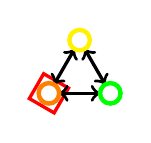
\begin{tikzpicture}[scale=0.26]]
%%%%%%%%%%%%%%%%%%%%%%%%%%%%%%%
% generated code
%%%%%%%%%%%%%%%%%%%%%%%%%%%%%%%
\draw [red, very thick, rotate around={60: (0, 0)}] (-0.7, -0.7) rectangle(0.7, 0.7);
%
\draw [very thick, <->] (0.25000000000000006, 0.4330127018922193) -- (1.25, 2.165063509461097) ;
\draw [very thick, <->] (1.75, 2.165063509461097) -- (2.75, 0.4330127018922193) ;
\draw [very thick, <->] (2.5, 0) -- (0.5, 0) ;
%
\draw [orange, ultra thick] (0,0) circle [radius= 0.5 ];
\draw [yellow, ultra thick] ( 1.5 , 2.59807621135 ) circle [radius= 0.5 ];
\draw [green,  ultra thick] ( 3.0 , 0 ) circle [radius= 0.5 ];
%%%%%%%%%%%%%%%%%%%%%%%%%%%%%%%
    \end{tikzpicture}
%\end{figure}
%
%
%%%%%
} average activity rate in a time bucket is calculated as

\begin{equation}
    \label{eq:rateEst}
    \bar{r} = \frac{N}{T},
\end{equation}
where $N$ is the number of activities in a bucket of time length $T$. Due to the statistical
variations in the number of activities in any given time interval, there exists an uncertainty in our 
estimate of this average rate. Figure~\ref{fig:confidence} illustrates this idea that as we continue to 
observe additional activities, our confidence in the underlying activity rate grows; the bounds shown 
are those of a 95\% confidence interval.



%%%%%
% figure
%
\begin{figure}[h]
	\begin{center}
		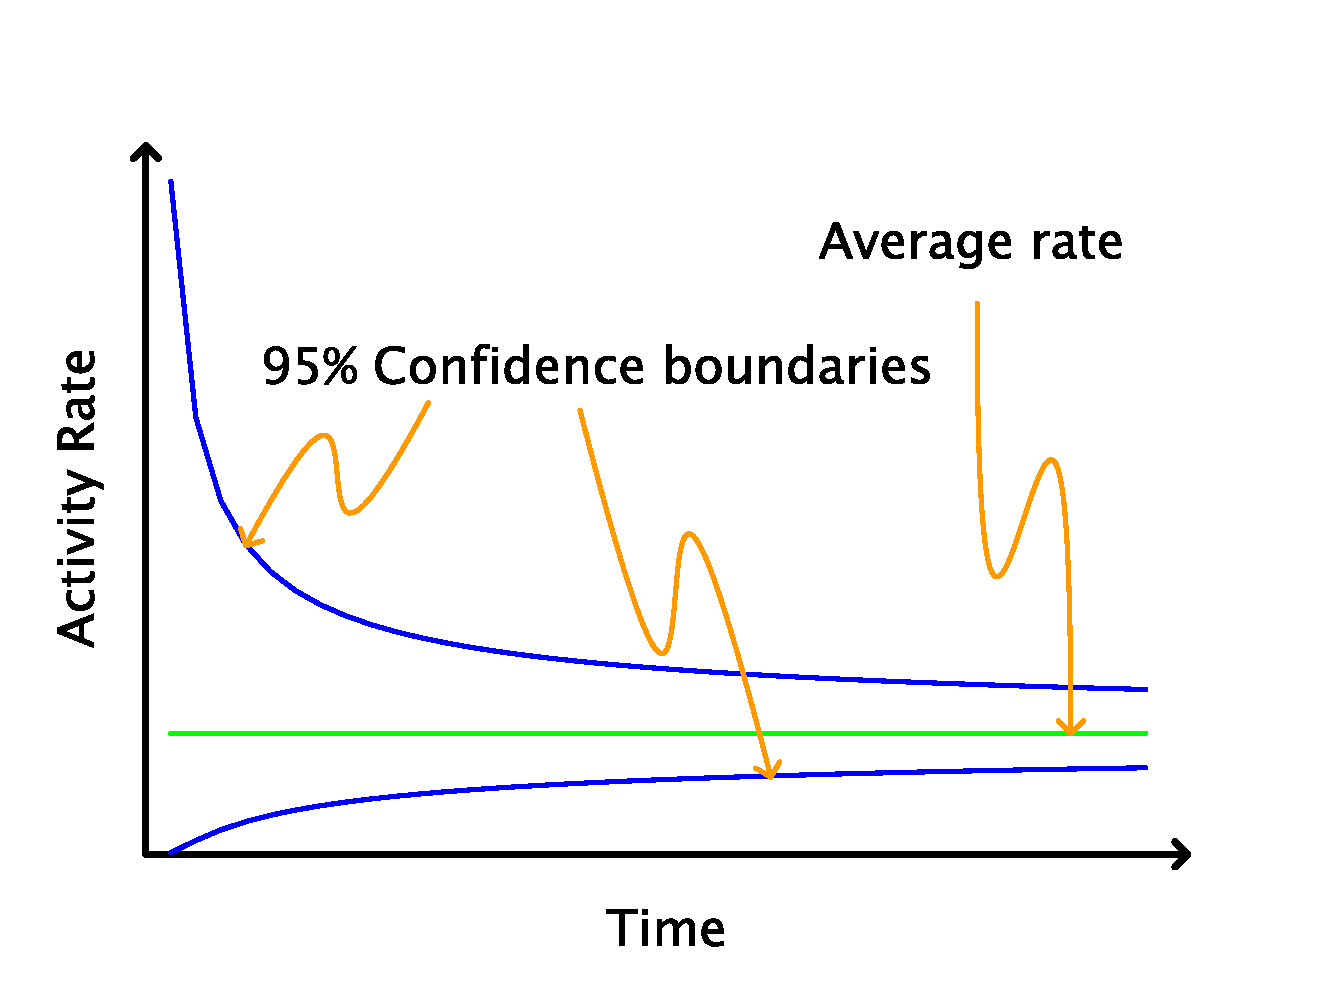
\includegraphics[width=3.5in]{./imgs/fig2.pdf}
	\end{center}
	\caption{The 95\% confidence interval (blue) representing the uncertainty in the estimated activity 
		rate (green) decreases in size as we observe additional activities. }
    	\label{fig:confidence}
\end{figure}
%
%
%%%%%

%Below, we will determine how many activities $N$ we need to count to estimate the average activity rate, $\bar{r}$, to a desired level
%of confidence (e.g. 95\%). In other words, we can ask: given a level of confidence, how wide is the range of uncertainty
%about the rate estimate?
%
%The details of calculating the confidence level can be found in the next section.  Next, we explore the connection between
%uncertainty in the rate estimate and the size of the signal we can detect.


%%%%%%%%%%%%%%%%%%%%%%%%%%%%%%%%%%
\subsection{Signal Sensitivity}
\label{sens}

%%%%%
% figure
%
\begin{figure}[h]
    \centering
    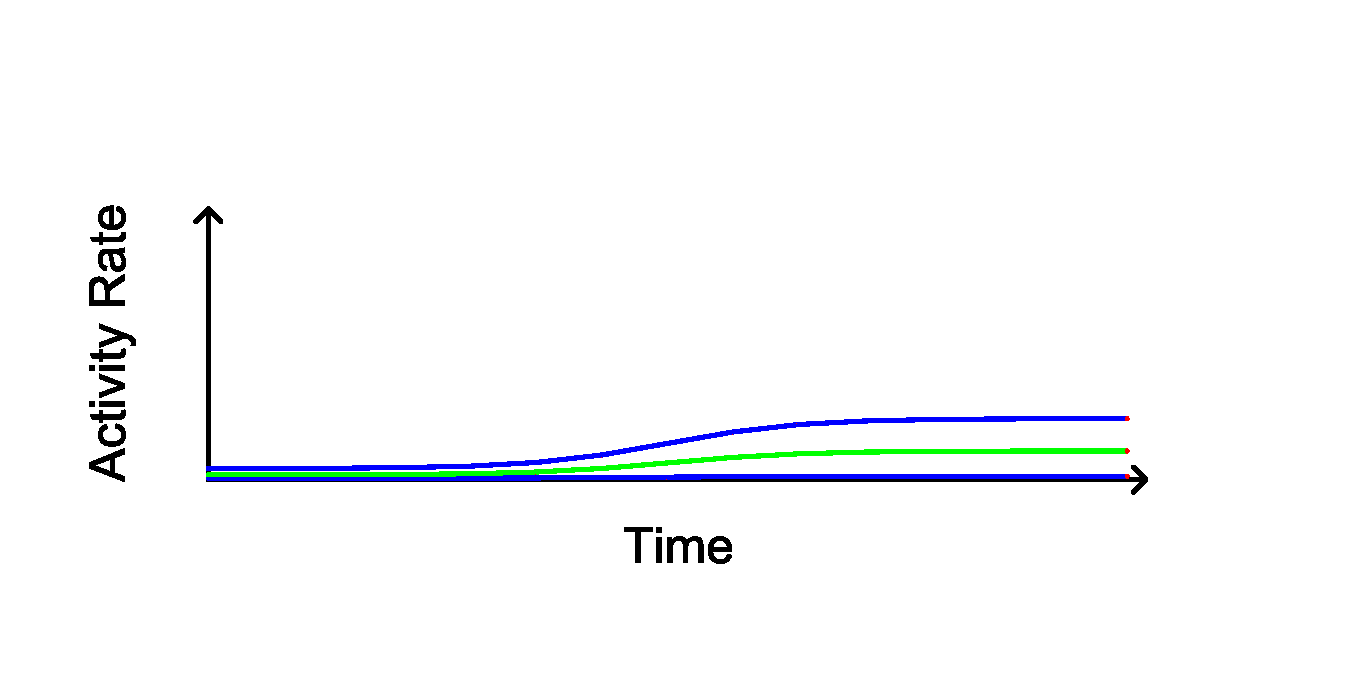
\includegraphics[width=3.5in]{./imgs/fig3a.pdf}
    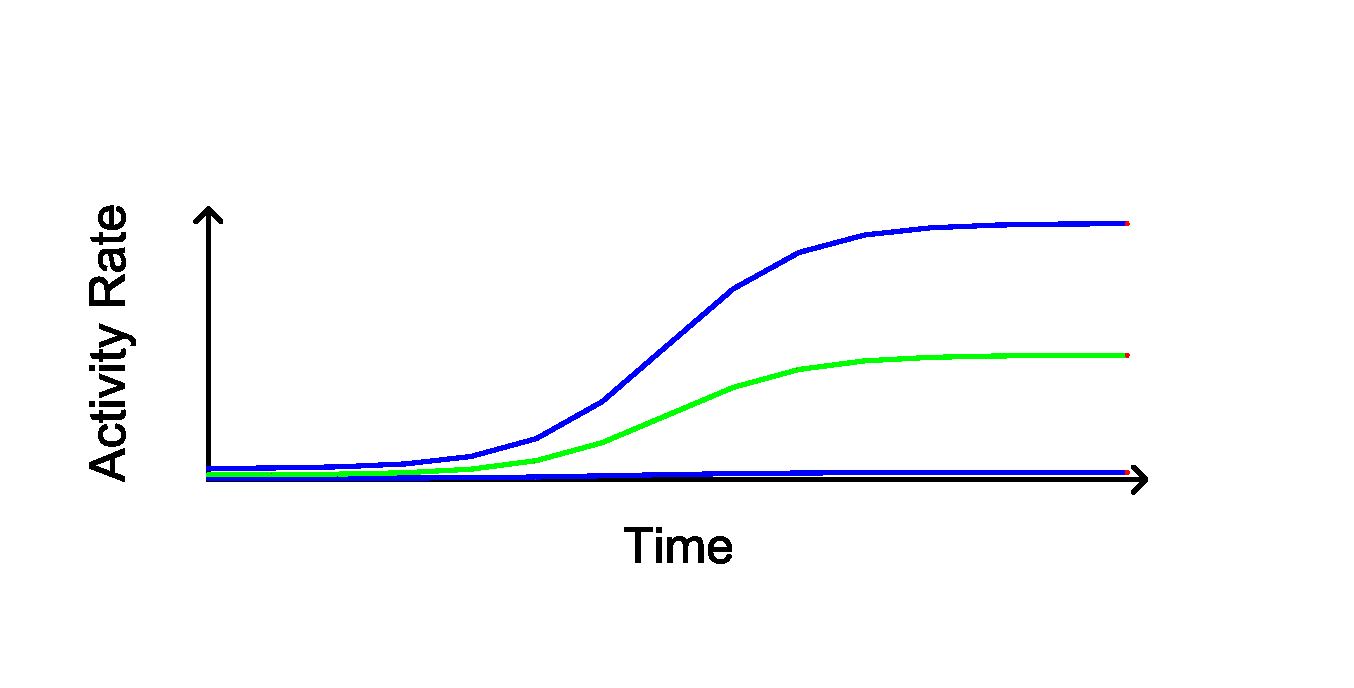
\includegraphics[width=3.5in]{./imgs/fig3b.pdf}
        \caption{A change in rate from the start time (left) to the end time (right) is established when the 
		change is equal to -- or greater than -- the uncertainty in the rate earlier estimate. The upper 
		image shows the point at which we cross this threshold. Before this criteria is met, the 
		change in rate remains within the uncertainty and observation of a signal is 
		indeterminate. The lower image shows this situation.}
    \label{fig:signal}
\end{figure}
%
%
%%%%%

%When
Higher
\reversemarginpar\marginpar{\raggedleft
%%%%%
% figure  ICON VIEW  SECTION 2.2
%
%\begin{figure}[!h]
    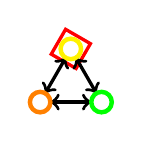
\begin{tikzpicture}[scale=0.26]]
\draw [red, very thick, rotate around={60: (1.5, 2.598076211353316)}] (0.8, 1.898076211353316) rectangle(2.2, 3.298076211353316);
%
\draw [very thick, <->] (0.25000000000000006, 0.4330127018922193) -- (1.25, 2.165063509461097) ;
\draw [very thick, <->] (1.75, 2.165063509461097) -- (2.75, 0.4330127018922193) ;
\draw [very thick, <->] (2.5, 0) -- (0.5, 0) ;
%
\draw [orange, ultra thick] (0,0) circle [radius= 0.5 ];
\draw [yellow, ultra thick] ( 1.5 , 2.59807621135 ) circle [radius= 0.5 ];
\draw [green,  ultra thick] ( 3.0 , 0 ) circle [radius= 0.5 ];
%%%%%%%%%%%%%%%%%%%%%%%%%%%%%%%
    \end{tikzpicture}
%\end{figure}
%
%
%%%%%
}
underlying activity rates lead naturally to more certain estimates of said rate than lower ones. 
For a low activity rate, it is possible that small changes in our estimated rate 
(calculated from one bucket to the next) will be inconclusive; the statistics of infrequent events 
lead to some amount of variation. In order to declare a valid signal, the variation due to e.g. 
infrequent events must be smaller than the thing we define as `signal.' Therefore, we observe
a valid signal in a time series when the activity rate between buckets has changed by 
more than the rate signal sensitivity, $\Delta r$, defined as

%%Consideration: when we talk about the change in activity rate, we're talking about a change between buckets; however, we do not specify which rate signal sensitivity we're using to compare. For two buckets, we see two singnal sensitivities. Options:
%%1.) We could average the two signal sensativities to compare with $\Delta r$
%%2.) We could de‎fine $\Delta r$ as the distance between uncertainty bounds between buckets and still continue to use the definition of signal as $\delta r$<<$\Delta r$.  


\begin{equation}
    \label{eq:signal}
    | r(t_f) - r(t_i) | \geq \Delta r.
\end{equation}

Each bucket size is defined by the difference between the variables $t_f$ and $t_i$, the times at which 
the activity rate is measured. The associated time duration $T_l = t_f - t_i$ is the signal latency.  


%%%%%%%%%%%%%%%%%%%%%%%%%%%%%%%%%%
\subsection{Signal Sensitivity--Confidence Criteria} 
\label{conf}


If  
\reversemarginpar\marginpar{\raggedleft
%%%%%
% figure  ICON VIEW SECTION 2.3
%
%\begin{figure}[!h]
    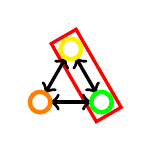
\begin{tikzpicture}[scale=0.26]]
\draw [red, very thick, rotate around={-60: (3.0, 0)}] (-0.7, -0.7) rectangle(3.7, 0.7);
%
\draw [very thick, <->] (0.25000000000000006, 0.4330127018922193) -- (1.25, 2.165063509461097) ;
\draw [very thick, <->] (1.75, 2.165063509461097) -- (2.75, 0.4330127018922193) ;
\draw [very thick, <->] (2.5, 0) -- (0.5, 0) ;
%
\draw [orange, ultra thick] (0,0) circle [radius= 0.5 ];
\draw [yellow, ultra thick] ( 1.5 , 2.59807621135 ) circle [radius= 0.5 ];
\draw [green,  ultra thick] ( 3.0 , 0 ) circle [radius= 0.5 ];
%%%%%%%%%%%%%%%%%%%%%%%%%%%%%%%
    \end{tikzpicture}
%\end{figure}
%
%
%%%%%
} 
we assume we are interested in estimating the activity rate (c.f. Equation~\ref{eq:rateEst}) of 
some form of steady-state process, the observed activities in any given period will be distributed 
about the long term mean. As for a typical Poisson process (discussed further in 
Section~\ref{poisson}), the span of fixed-percentage confidence intervals decreases with an 
increasing number of observed activities, and as mentioned in Section~\ref{sens}, this uncertainty 
also inversely scales with the underlying activity rate.

Referring to the signal definition in Equation~\ref{eq:signal}, we can establish a rough criteria for 
confidence in terms of the signal uncertainty, $\delta r$:

%\begin{equation}
%    \label{eq:criteria}
%    \frac{\delta r}{\bar{r}_{max}} << \frac{\Delta r}{\bar{r}_{max}}.
%\end{equation}
%where $\bar{r}_{max}$ will be the lower rate estimate (initial if detecting rising activity rate 
%but final if detecting falling activity rate).

% rename r_max to r_low for simpler explanation
\begin{equation}
    \label{eq:criteria}
    \frac{\delta r}{\bar{r}_{low}} << \frac{\Delta r}{\bar{r}_{low}}.
\end{equation}
where $\bar{r}_{low}$ will be the lower activity rate estimates of the two observations. The 
duplicate denominator exists to emphasize the fact that although the span of the 
confidence interval increases with more activities, the relative interval size decreases. 
% can make this ^ more clear the relative interval size is discussed in a later section

To make this inequality a bit more concrete, we can introduce a criteria factor, $\eta$, which 
specifies the relative size difference between our observed rate change (i.e. potential signal) 
and the relative uncertainty interval,

%\begin{equation}
%    \label{eq:criteriaParam}
%    \frac{\delta r}{\bar{r}_{max}} = \frac{\eta \Delta r}{\bar{r}_{max}}
%\end{equation}

% similar replacement, as above
\begin{equation}
    \label{eq:criteriaParam}
    \frac{\delta r}{\bar{r}_{low}} \eta  = \frac{\Delta r}{\bar{r}_{low}},
\end{equation}
where $\eta \ge 1$.

We will sometimes refer to the right-hand side of Equation~\ref{eq:criteriaParam} as our `signal 
sensitivity', and the left-hand side as a `relative (confidence) interval size'. Flexibility in the 
choice of $\eta$ allows us to prioritize high-certainty classification of signal 
(larger $\eta$, greater separation of observed signal and uncertainty bounds, 
typically requiring longer observation time), or lower-certainty classification (smaller $\eta$, 
less signal-uncertainty separation, typically requiring shorter observation time).


%%%%%%%%%%%%%%%%%%%%%%%%%%%%%%%%%%%%%%%%%%%%%%%%%%%%%%%%%%%%%%%%%%%
\section{Statistics of Time Series of Activities} 
\label{time}

In this section, we explore some of the underlying mathematics and statistics involved in 
activity rate estimation. The goal is to demonstrate a method for calculating confidence 
intervals for rate estimates, and how to consider the available tradeoffs inherent in such 
a measurement.


%%%%%%%%%%%%%%%%%%%%%%%%%%%%%%%%%%
\subsection{Poisson Activity Probability} 
\label{poisson}

Because 
\reversemarginpar\marginpar{\raggedleft
%%%%%
% figure  ICON VIEW  SECTION 2.1 and 3.1
%
%\begin{figure}[!h]
    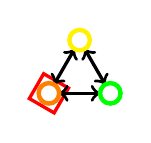
\begin{tikzpicture}[scale=0.26]]
%%%%%%%%%%%%%%%%%%%%%%%%%%%%%%%
% generated code
%%%%%%%%%%%%%%%%%%%%%%%%%%%%%%%
\draw [red, very thick, rotate around={60: (0, 0)}] (-0.7, -0.7) rectangle(0.7, 0.7);
%
\draw [very thick, <->] (0.25000000000000006, 0.4330127018922193) -- (1.25, 2.165063509461097) ;
\draw [very thick, <->] (1.75, 2.165063509461097) -- (2.75, 0.4330127018922193) ;
\draw [very thick, <->] (2.5, 0) -- (0.5, 0) ;
%
\draw [orange, ultra thick] (0,0) circle [radius= 0.5 ];
\draw [yellow, ultra thick] ( 1.5 , 2.59807621135 ) circle [radius= 0.5 ];
\draw [green,  ultra thick] ( 3.0 , 0 ) circle [radius= 0.5 ];
%%%%%%%%%%%%%%%%%%%%%%%%%%%%%%%
    \end{tikzpicture}
%\end{figure}
%
%
%%%%%
}
social activities (e.g. Tweets) are timed approximately randomly and have inter-activity 
times which follow an exponential distribution, we can classify such a process as a Poisson 
process. As such, we can model the probability of observation times $t$ between events as 

\begin{equation}
    \label{eq:tbe}
    p_{activity}(t) = r e^{-r t}.
\end{equation}

This leads to the probability of observing $n$ activities in time $t$, and with activity rate $r$, 
following a Poisson distribution:
\begin{equation}
    \label{eq:poisson}
    P(n) = \frac{e^{-r t} (r t)^n}{n!}.
\end{equation}
The expected value of this distribution $E[n]=n=rt$. The mean and variance of the Poisson distribution are 
both equal to $r$\cite{tbd}.



%%%%%%%%%%%%%%%%%%%%%%%%%%%%%%%%%%
\subsection{Poisson Confidence Intervals} 
\label{conf}

We 
\reversemarginpar\marginpar{\raggedleft
%%%%%
% figure  ICON VIEW SECTION 3.2
%
%\begin{figure}[!h]
    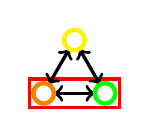
\begin{tikzpicture}[scale=0.26]]
\draw [red, very thick, rotate around={0: (0, 0)}] (-0.7, -0.7) rectangle(3.7, 0.7);
%
\draw [very thick, <->] (0.25000000000000006, 0.4330127018922193) -- (1.25, 2.165063509461097) ;
\draw [very thick, <->] (1.75, 2.165063509461097) -- (2.75, 0.4330127018922193) ;
\draw [very thick, <->] (2.5, 0) -- (0.5, 0) ;
%
\draw [orange, ultra thick] (0,0) circle [radius= 0.5 ];
\draw [yellow, ultra thick] ( 1.5 , 2.59807621135 ) circle [radius= 0.5 ];
\draw [green,  ultra thick] ( 3.0 , 0 ) circle [radius= 0.5 ];
%%%%%%%%%%%%%%%%%%%%%%%%%%%%%%%
    \end{tikzpicture}
%\end{figure}
%
%
%%%%%
}
are counting activities within a defined time interval in order to estimate the activity rate $\bar{r}$. 
Confidence intervals for the Poisson distribution with confidence level equal to $100\%(1-\alpha)$ 
are given by \cite{George:2012},

\begin{equation}
    \label{eq:chisqconf}
    \frac{1}{2T} \chi^2(\alpha/2;2n) \leq r \leq \frac{1}{2T} \chi^2(1-\alpha/2;2n+2)
\end{equation}
where $\chi^2$ is the inverse cumulative distribution function, $CDF^{-1}(p; n)$, of the $\chi^2$ 
distribution.\footnote{A useful approximation to the exact interval is given by:

$[ n(1 - \frac{1}{9n} - \frac{z_{\alpha}}{3\sqrt{n}})^3 , 
(n+1)(1- \frac{1}{9(n+1)} + \frac{z_{\alpha}}{3\sqrt{n+1}})^3]$ }
Note that with this definition of $\alpha$, a confidence interval of 90\% corresponds to 
$\alpha=0.1$. Example $90\%$ confidence intervals and their relative sizes are shown in 
Table~\ref{tab:conf}.

To determine the parameters satisfying our data collection goals, we can find the value of $n$ for 
which the time interval and confidence level match our requirements for signal detection.  
That is, we can now calculate any one of signal sensitivity, signal latency, activity rate, or confidence 
level given the other parameters. Example calculations for various design choices are illustrated in the 
last section of this paper.

%%%%%
% table: poisson intervals
%
\begin{table}[!h]\centering
    \begin{tabular}{r|x{3.5cm}|c|c}
     \hline
$n$ & Interval Bounds & Interval Size ($\delta n$) & Relative Interval\\ 
\hline 
1 &   0.0513, 4.744  & 4.693 & 4.693\tabularnewline 
2 &   0.3554, 6.296  & 5.940 & 2.970\tabularnewline 
3 &   0.8177, 7.754  & 6.936 & 2.312\tabularnewline 
4 &   1.366, 9.154  & 7.787 & 1.947\tabularnewline 
5 &   1.970, 10.51  & 8.543 & 1.709\tabularnewline 
6 &   2.613, 11.84  & 9.229 & 1.538\tabularnewline 
7 &   3.285, 13.15  & 9.863 & 1.409\tabularnewline 
8 &   3.981, 14.43  & 10.45 & 1.307\tabularnewline 
9 &   4.695, 15.71  & 11.01 & 1.223\tabularnewline 
10 &   5.426, 16.96  & 11.54 & 1.154\tabularnewline 
20 &   13.25, 29.06  & 15.81 & 0.7904\tabularnewline 
30 &  21.59, 40.69  & 19.10 & 0.6366\tabularnewline 
40 &  30.20, 52.07  & 21.87 & 0.5468\tabularnewline 
50 &  38.96, 63.29  & 24.32 & 0.4864\tabularnewline 
60 &  47.85, 74.39  & 26.54 & 0.4423\tabularnewline 
70 &  56.83, 85.40  & 28.57 & 0.4082\tabularnewline 
80 &  65.88, 96.35  & 30.47 & 0.3809\tabularnewline 
90 &  74.98, 107.2  & 32.25 & 0.3584\tabularnewline 
100 &  84.14, 118.1  & 33.94 & 0.3394\tabularnewline 
200 &  177.3, 224.9  & 47.55 & 0.2378\tabularnewline 
300 &  272.1, 330.1  & 58.00 & 0.1933\tabularnewline 
400 &  367.7, 434.5  & 66.82 & 0.1670\tabularnewline 
500 &  463.8, 538.4  & 74.58 & 0.1492\tabularnewline 
750 &  705.5, 796.6  & 91.11 & 0.1215\tabularnewline 
1000 &  948.6,  1054.  & 105.0 & 0.1050\tabularnewline 
\end{tabular}
\caption{$90\%$ ($\alpha$ = 0.1) confidence intervals around the number of events counted, 
$n$, in unit time $T$. Rate interval size is $\delta r = \delta n/T$. Note that while the 
absolute size of the interval increases, the relative interval uncertainty decreases.}
\label{tab:conf}
\end{table}
%
%%%%%



%%%%%%%%%%%%%%%%%%%%%%%%%%%%%%%%%%
%\subsection{Confidence Interval Approximations and Bucketed Activity Counts}
\subsection{Normal Approximations and Bucketed Counts}
\label{confapprox}

%\subsubsection{Frequent Activities} 

For a sufficiently large number of observed activities (equivalently, if the activity rate is sufficiently 
large), the Poisson distribution can be approximated by a normal distribution. For example, 
the common $95\%$ confidence interval is symmetric about the mean and given by

\begin{equation}
    \label{eq:largenconf}
    \bar{r} - 1.96 \sqrt{\bar{r}/n} \leq \hat{r} \leq \bar{r} + 1.96 \sqrt{\bar{r}/n}.
\end{equation}
Depending on our particular use-case or desire for accuracy, use of a normal confidence interval 
may be sufficient -- or at least a fast approximation.

%\subsubsection{Bucketed Activity Counts}

For various reasons, activity counts may be collected in buckets of some pre-defined time length.  
Estimation of the activity rate may by more naturally calculated by bucket than by total time $T$ 
(e.g. as required by our confidence requirements). In general, the relationship between total time 
$T$ and (constant) bucket size $\Delta t$ is 

\begin{equation}
    \label{eq:bucket}
    \Delta t = \frac{T}{k}
\end{equation}
where $k$ is the number of buckets. This parameter can also be used to calculate a corresponding 
signal latency -- in units of `buckets' -- $k_l = T_l/\Delta t$.

In the case where $\Delta t << T$, resolution times are typically interchangeable with the number 
of buckets. However, in general, the bucket resolution time will not be an even multiple of the 
bucket size. In this case, the need for a calculation of average activity rate per bucket 
$\bar{r} = n/\Delta t$ adds another layer of variability and is beyond the scope of this 
work. 


%%%%%%%%%%%%%%%%%%%%%%%%%%%%%%%%%%
\subsection{Summary of Trade-Offs and Parameters}
\label{tradoffs}

When 
\reversemarginpar\marginpar{\raggedleft
%%%%%
% figure  ICON VIEW SECTION 3.4
%
%\begin{figure}[!h]
    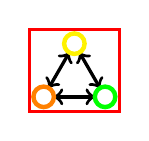
\begin{tikzpicture}[scale=0.26]]
\draw [red, very thick, rotate around={0: (0, 0)}] (-0.7, -0.7) rectangle(3.7, 3.298076211353316);
%
\draw [very thick, <->] (0.25000000000000006, 0.4330127018922193) -- (1.25, 2.165063509461097) ;
\draw [very thick, <->] (1.75, 2.165063509461097) -- (2.75, 0.4330127018922193) ;
\draw [very thick, <->] (2.5, 0) -- (0.5, 0) ;
%
\draw [orange, ultra thick] (0,0) circle [radius= 0.5 ];
\draw [yellow, ultra thick] ( 1.5 , 2.59807621135 ) circle [radius= 0.5 ];
\draw [green,  ultra thick] ( 3.0 , 0 ) circle [radius= 0.5 ];
%%%%%%%%%%%%%%%%%%%%%%%%%%%%%%%
    \end{tikzpicture}
%\end{figure}
%
%
%%%%%
}
underlying activity rates are high, we can make highly-certain estimates of the rate in a relatively 
short time. This also allows us to detect small changes in a previous activity rate (high signal 
sensitivity). Similarly, lower activity rates lead to larger uncertainty in our estimates and require that 
we observe for a longer period of time to establish the existance of a signal at the same 
level of confidence. Along with some example use-case goal/action suggestions, these model 
trade-offs are summarized in Table~\ref{tab:tradeoff}.

For additional reference, Table~\ref{tab:summary} includes a summary of the model parameters 
introduced in this work.


%% added whitespace to this tex to make the compiled table easier to read
%%%%%
% table: model trade-offs
%
\begin{table}[!h]
    \begin{tabular}{ p{3.0cm}| p{5.2cm} | p{2.6cm}}
     \hline
Goal  & Possible Actions & Example\\
\hline
Minimize activities 

(i.e. decrease $n$)  & 

increase $\Delta r$ (decrease signal sensitivity); decrease confidence factor ($\alpha$); 
	increase $T_l$ (wait longer for the signal)  & Section~\ref{ex:1} 

(large signal latency) \\

\hline	
Increase signal sensitivity 

(i.e. decrease $\Delta r$) & 

increase $T$ (increase number of buckets ($k$); increase bucket size ($\Delta t$) ); increase activity 
	rate ($r$) by broadening filter or increase PowerTrack sampling & Section~\ref{ex:3} 

(sensitivity with high rate) \\

\hline
Decrease signal latency  

(i.e. decrease $T_l$) & 

decrease signal sensitivity $\Delta r$; decrease confidence factor ($\alpha$); increase activity 
	rate ($r$) by broadening filter or increase PowerTrack sampling & Section~\ref{ex:2} 

(large signal latency) \\

\hline
Decrease signal uncertainty 

(i.e. decrease $\eta$) & 

increase $T$ [increase number of buckets ($k$); or increase bucket size ($\Delta t$) ); increase 
	activity counts (increase $n$, $r$) by broadening filter; increase PowerTrack sampling & 
	Section~\ref{ex:2} 

(small $\eta \le 1)$ \\
\hline
\end{tabular}
\caption{Summary of model trade-offs.}
\label{tab:tradeoff}
\end{table}
%
%%%%%


%%%%%
% table: model parameters
%
\begin{table} [!h]
    \begin{tabular}{p{3.0cm}| p{1.9cm}|p{5.9cm}}
     \hline
Parameter  & Symbol & Definition \\
\hline	
Activity count & $n$ & Number of activities in time $T$\\
Sample time & $T$	& Duration of observation\\
Activity rate & $r$	& Number of activities per time $T$\\
Avg. activity rate & $\bar{r} = n/T$ & Our estimate of average activity rate \\
Rate uncertainty & $\delta r$	& Uncertainty of our rate estimate \\
Confidence factor & $\alpha$ & Confidence level is $100\% (1-\alpha)$\\
Signal sensitivity & $\Delta r=r_{f}-r_{i}$ & Detectable change in activity rate \\
Signal latency & $T_l$ & Time required to detect $\Delta r$  \\
Criteria factor & $\eta$ & Rate signal criteria multiplier factor (i.e. $\eta = 3$ means 
	relative signal is $3 \times$ random variations in sample) \\
Bucket size & $\Delta t$ & Predetermined time scale for estimating rate (possibly already determined in your system)\\
Number of buckets & $k=T/\Delta t$ & Observation duration expressed in number of buckets \\
Sampling operator & $S$	& PowerTrack sampling operator (e.g. ``sample:$S$'') \\
\hline
\end{tabular}
\caption{Summary of model parameters.}
\label{tab:summary}
\end{table}
%
%%%%%


%%%%%%%%%%%%%%%%%%%%%%%%%%%%%%%%%%%%%%%%%%%%%%%%%%%%%%%%%%%%%%%%%%%
\section{Example Calculations} 
\label{examples}



%%%%%%%%%%%%%%%%%%%%%%%%%%%%%%%%%%
\subsection{Estimate PowerTrack Sampling Operator Value} 
\label{ex:1}

Recall that the sampling operator allows us to reduce the full firehose of activities to a representative 
subset of user-defined size. Selecting the value of $S$ is a process that often starts at $S =100\%$.  
By monitoring the number of activities, $n$, that are filtered through the rules, we get an 
estimate for $\bar{r}$.

Assume that using 100\% of the firehose for one minute, we observe $n = 10$ activities. Further, assume 
that we would like to detect a change in activity rate from 10 to 20 activities per minute using 
$\eta = 3$. What value of $S$ should we choose to sample from the firehose?

Imagine for this example that we are comfortable with a signal latency of two days -- i.e. our system 
needs to react to signals in about two days. Given that we expect 10 activities per minute or 
14,400 activities per day, we need to ensure we meet our signal sensitivity criteria:
\begin{equation}
\label{eq:ex1:criteria}
\frac{\delta r}{\bar{r}} = \text{Relative Interval Size} = 
	\frac{1}{3} 
	\frac{(20-10) \text{ activities}}{\text{min}} 
	\frac{1 \text{ min}}{10 \text{ activities}} = \frac{1}{3} 
\end{equation}
over this two-day period. Table~\ref{tab:conf} requires about 100 activities (total, over the two days) 
for a relative interval size of $1/3 \approx 33\%$. Hence, instead of using $100\%$ of the 
firehose, we can use $S = \frac{100}{28,800} << 1\% \rightarrow 1\%$\footnote{Recall from 
Section~\ref{filter} that the sampling operator has a precision of $1\%$}.



   
%%%%%%%%%%%%%%%%%%%%%%%%%%%%%%%%%%
\subsection{Estimate Signal Latency} 
\label{ex:2}


Imagine we observe rate of 10 activities per minute and we want to detect a change in activity 
rate from 10  to 20 activities per minute.  If we again use a value of $\eta = 3$, how long 
does it take to identify such a change in 
the activity rate as a signal with 90\% confidence level? To calculate an answer, we use the 
signal sensitivity--Confidence Criteria, Equation~\ref{eq:criteriaParam} and Confidence Interval 
Sizes from Table \ref{tab:conf}.

With a criteria factor of 3, our signal sensitivity is
\begin{equation}
\label{eq:ex2:latency}
\frac{1}{\eta} \frac{\Delta r}{\bar{r}} = 	
	\frac{1}{3} 
	\frac{(20-10) \text{ activities}}{\text{min}} 
	\frac{1 \text{ min}}{10 \text{ activities}} = \frac{1}{3} \approx 33\%,
\end{equation}
and with $n = 10$, our $90\%$ confidence interval size is about 11.54 (cf. Table~\ref{tab:conf}). 

Comparing the confidence interval size to our signal sensitivity,
\begin{equation}
    \label{eq:ex2:notmet}
    \frac{\delta r}{\bar{r}} = \frac{(11.54)}{10} \approx 115.4\% \not\le 33\%, 
\end{equation}
we can see that we cannot detect an increase in rate of 10 activities per minute after just one 
minute.

To determine our signal latency, $T_l$, we use the signal sensitivity calculated above and 
Table~\ref{tab:conf} to find the approximate number of activities we must observe to meet our 
criteria. To ensure our relative confidence interval matches our signal sensitivity at $33\%$, we 
see that we must observe approximately 100 activities. Since our previous rate, $\bar{r}_{low}$ 
was 10 activities per minute, we determine that it will require $T_l = 10$ minutes of 
observation to detect our desired change in signal.


%% original BL calc
%Imagine we observe rate of 10 activities per minute and we want to detect a change in activity rate of 20 activities
%per minute.  How long does it take to identify a change in the activity rate as a signal with 90\% confidence level? 
%To calculate an answer, we will be using the signal sensitivity--Confidence Criteria, \ref{eq:criteriaParam} and 
%Confidence Interval Sizes from Table \ref{tab:conf}
%
%\begin{itemize}
%\item Calculating $T_{l}$
%\item Signal criteria factor $\eta=\frac{1}{3}$ -- In this case we choose a criteria that reflects our wish to see fewer false positives.
%\item Signal Sensitvity $\frac{\eta \Delta r}{\bar{r}} = \frac{1}{3}\frac{(20-10)}{min} \frac{1 min}{10 activities}= 33\%$
%\item Confidence Interval Size at $N =10$ is $11.54$. %Confidence intervals around $\r_bar$ only depend on N. 
%\end{itemize}
%
%It is clear that we cannot detect a change in activity rate of 10 activities/minute by measuring for only 1 min.  Notice that our criteria is not fulfilled:
%\begin{equation}
%    \label{eq:ex2:notmet}
%    \frac{\delta r}{\bar{r}} = \frac{(11.54)}{10} \approx 115.4\% \not\le 33\% 
%\end{equation}
%
%The time $T_{l}$ that it takes to observe this signal $\Delta r =20$ with signal criteria factor of $\eta=\frac{1}{3}$ depends 
%on the total number of activities $N_t$ that we must observe to have a credible estimate of the activity rate. Because activities 
%are infrequent, we will look up the confidence interval size, synonymous to $\delta r$, for small numbers of activities 
%in Table \ref{tab:conf}.  As $N_t$ increases, the relative $90\%$ confidence interval size narrows around the 
%average rate, which can be seen through the decreasing relative interval value in Table \ref{tab:conf}.  We need to 
%find the value for $N_t$.
%
%We can only detect a signal $\Delta r$ when our signal criteria is fulfilled:
%\begin{equation}
%    \label{eq:ex2:met}
%    \frac{\delta r}{\bar{r}} = \text{ Relative Interval Size} = 33\% =  \frac{\eta \Delta r}{\bar{r}}
%\end{equation}
%
%You can look up the required Relative Interval Size in Table $\ref{tab:conf}, 100\%/3 = 33\%$ to see
%that we need to observe at least 100 events on average to reach our criteria. Therefore, $T_l = 10 \text{ minutes}$ because
%we will have observed $100$ activities in $10$ minutes given $\bar{r} = \frac{10 \text{ activities}}{1 \text{ min}}$. That is, we 
%must observe 10 minutes of activities to detect our desired signal.


%%%%%%%%%%%%%%%%
%How long does it take to identify a change in the activity rate as a signal?
%
%As an example for calculating $T_{l}$, we choose a specific signal $\Delta r = \frac{10}{T}$.  The time $T_{l}$ that it takes to observe this signal $\Delta r$, or equivalently, the number of buckets, $k$, depends the total number of activities $N_t$ that we must observe to have a credible estimate of the activity rate. Because activities are infrequent, we will look up the confidence interval for small numbers of activities this up in Table \ref{tab:conf}.  As $N_t$ increases, the $90\%$ confidence interval length $I$ narrows around the average rate $\delta r$ decreases.  See Equation \ref{...}3??.  We need to find the value for $N$ at which point $\delta r$ has decreased enough to allow us to see our signal $\Delta r = \frac{10}{T}$.  
%
%Choosing $\eta=1$, we see in Table \ref{tab:conf} that for $\Delta r = \frac{10}{T}$, we must have $N\geq7$ causing $I > 10\eta$ in order to observe our signal.  Notice that $N_t=7$ is the point after which we could first observe a signal.  Thus, we say that $T_{l}>T_{N_t}$ defines the time that it takes to observe a signal, which means that signal latency is greater than the amount of time that it takes to collect $N_t$ activities.  Takes 2 periods to get the calculation> have to calculate the rate in the first then the second and compare.
%
%We can decrease $T_{l}$ in several ways.  First, we could try improving the rate at which we achieve $N_t$ by  increasing our PowerTrack sampling.  Otherwise, we could decrease $T_{l}$ as we narrow $I$ through a lower confidence level $(1-\alpha)$.  The lower confidence level tightens $I$ around smaller $N$ allowing the potential signal to become clearer faster, but this goal is accomplished at the cost of decreased confidence.  Another basic option is to simply choose a smaller (larger?) signal size such as $\Delta r = \frac{5}{T}$ from our previous example.  All of these strategies would decrease $T_{l}$.



%%%%%%%%%%%%%%%%%%%%%%%%%%%%%%%%%%
\subsection{Estimate Signal Sensitivity}
\label{ex:3}

Suppose we would like to determine the magnitude of a signal change needed to 
classify it as significant. 
As shown in Equation~\ref{eq:criteriaParam}, 
classifying a signal $\Delta r$ as significant depends on the choice of criteria factor 
$\eta$ and the observation parameters that determine the uncertainty $\delta r$. 
Specifically, we will need to choose a criteria factor $\eta$ and confidence level 
$(1-\alpha)$, and our observation will be characterized by total activity count $n$ 
and total time $T$.

Let us assume we have decided to classify as significant a signal with $\eta = 10$, or 
$\Delta r = 10 \times \delta r$. Furthermore, we have chosen a 90\% confidence interval 
and observed $n$=10,000 activities over a period of $T$=1 minute 
(60 seconds) for an estimated rate of $\bar r = 167$ activities per second. We use 
Equation~\ref{eq:chisqconf} to calculate the interval of activities for our 
90\% confidence level, and divide by observation period $T$ to obtain the corresponding 
minimum significant rate $\delta r = 5$ activities per second. Recall, however, 
that we have also specified a criteria factor $\eta = 10$. Therefore, in this example, 
in order to classify the change in rate as significant, we must observe a change at the 
level of $\Delta r =\eta \times \delta r = 10 \times 5 = 50$ activities per second. 
For an increasing activity rate, this corresponds to a total activity rate of 
$167 + 50 = 217$ activities per second. For a decreasing 
rate, 117 activities per second.


%Let us assume we have decided to classify as significant a signal with $\eta = \frac{1}{10}$, or 
%$\delta r = \frac{1}{10}\Delta r$. Furthermore, we have chosen a 90\% confidence interval 
%($\alpha = 0.1$), and observed $N$=10,000 activities over a period of $T$=1 minute 
%(60 seconds) for an estimated activity rate of $\bar r = 167~\si{\per\second}$. We next use 
%Equation~\ref{eq:chisqconf} to calculate the interval of activities for our 
%90\% confidence level, and divide by observation period $T$ to obtain the corresponding 
%minimum significant activity rate $\delta r = 5~\si{\per\second}$. Recall, however, 
%that we have also specified a criteria factor $\eta = 10$. Therefore, in this example, 
%in order to classify the change in rate as significant, we must observe a change at the 
%level of 
%$\Delta r =\frac{1}{\eta} \delta r = 10 (5~\si{\per\second}) = 50~\si{\per\second}$. 
%For an increasing activity rate, this corresponds to a total activity rate of 
%$167~\si{\per\second} + 50~\si{\per\second} = 217~\si{\per\second}$. For a decreasing 
%rate, $117~\si{\per\second}$.



% Procedure for this calculation:
% 	Using the tables.py script, calculate poisson_bounds1() for N=10000, confidence=0.90, 
% 	and the resulting bounds (to one decimal) are [9836.1, 10166.1]. This is an interval of count 
%	of activities; the corresponding bounds on the rate are given by this interval divided by 
% 	the time period, T=60 s: (10166.1-9836.1)/60 ~ 5 /s. 



%%%%%%%%%%%%%%%%%%%%%%%%%%%%%%%%%%%%%%%%%%%%%%%%%%%%%%%%%%%%%%%%%%%
\section{Conclusion} 

This work is intended to enable more confident analysis and understanding of the social data 
streams available through Gnip. A better understanding of the parameter trade-offs involved 
in any sort of measurement will hopefully empower you to use these data more efficiently in 
your own environment.

The latest version of this document and supporting code for creating figures and tables 
can be found at:

\noindent \url{https://github.com/DrSkippy27/Gnip-Realtime-Social-Data-Sampling}.

If you find errors in this work, or have comments, please email shendrickson@gnip.com. This 
work is licensed under a Creative Commons Attribution-ShareAlike 3.0 Unported License:

\noindent \url{http://creativecommons.org/licenses/by-sa/3.0/deed.en_US}.

%%%%%%%%%%%%%%%%%%%%%%%%%%%%%%%%%%%%%%%%%%%%%%%%%%%%%%%%%%%%%%%%%%%

\begin{thebibliography}{2013}



\bibitem[Mor13]{Morstatter:2013} F. Morstatter, J. Pfeffer, J. Liu, K. Carley, \textsl{Is the Sample Good Enough? Comparing Data from Twitter’s Streaming API with Twitter’s Firehose}, \url{http://www.public.asu.edu/~fmorstat/paperpdfs/icwsm2013.pdf} 2013.

\bibitem[Geo12]{George:2012} F. George B. Golam Kibria, \textsl{Confidence Intervals for Signal to Noise Ratio of
a Poisson Distribution}, \url{http://thescipub.com/abstract/10.3844/amjbsp.2011.44.55} 2013.

\end{thebibliography}

\end{document}
